
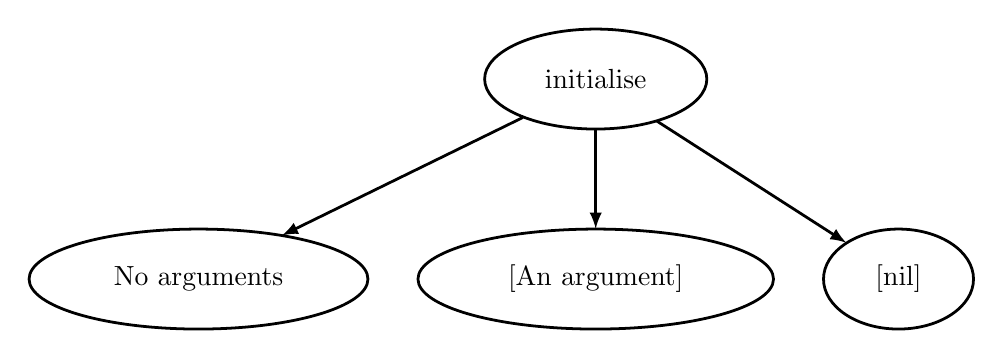
\begin{tikzpicture}[>=latex,line join=bevel,]
  \pgfsetlinewidth{1bp}
%%
\pgfsetcolor{black}
  % Edge: initialise -> a1
  \draw [->] (177.77bp,76.161bp) .. controls (156.04bp,65.521bp) and (124.82bp,50.241bp)  .. (91.021bp,33.696bp);
  % Edge: initialise -> a3
  \draw [->] (226.06bp,74.834bp) .. controls (243.27bp,63.78bp) and (267.27bp,48.365bp)  .. (294.24bp,31.046bp);
  % Edge: initialise -> a2
  \draw [->] (204bp,71.697bp) .. controls (204bp,63.983bp) and (204bp,54.712bp)  .. (204bp,36.104bp);
  % Node: a1
\begin{scope}
  \definecolor{strokecol}{rgb}{0.0,0.0,0.0};
  \pgfsetstrokecolor{strokecol}
  \draw (61bp,18bp) ellipse (61bp and 18bp);
  \draw (61bp,18bp) node {No arguments};
\end{scope}
  % Node: initialise
\begin{scope}
  \definecolor{strokecol}{rgb}{0.0,0.0,0.0};
  \pgfsetstrokecolor{strokecol}
  \draw (204bp,90bp) ellipse (40bp and 18bp);
  \draw (204bp,90bp) node {initialise};
\end{scope}
  % Node: a3
\begin{scope}
  \definecolor{strokecol}{rgb}{0.0,0.0,0.0};
  \pgfsetstrokecolor{strokecol}
  \draw (313bp,18bp) ellipse (27bp and 18bp);
  \draw (313bp,18bp) node {[nil]};
\end{scope}
  % Node: a2
\begin{scope}
  \definecolor{strokecol}{rgb}{0.0,0.0,0.0};
  \pgfsetstrokecolor{strokecol}
  \draw (204bp,18bp) ellipse (64bp and 18bp);
  \draw (204bp,18bp) node {[An argument]};
\end{scope}
%
\end{tikzpicture}

